\documentclass[a4paper, 11pt, pdftex, fleqn]{article}
\usepackage[utf8]{inputenc}
\usepackage[ngerman]{babel}
\usepackage{coordsys,logsys,color}
\usepackage{fancyhdr}
\usepackage[ngerman]{hyperref}
\usepackage{texdraw}
\usepackage{graphicx}
\usepackage{caption}

\NeedsTeXFormat{LaTeX2e}
\definecolor{darkblue}{rgb}{0,0,.6}
\hypersetup{colorlinks=true, breaklinks=true, linkcolor=darkblue, menucolor=darkblue, urlcolor=darkblue, citecolor=darkblue}

\setlength{\headheight}{15pt}
\pagestyle{fancy}

\renewcommand{\familydefault}{cmss}

\definecolor{fgcgray}{rgb}{0.4, 0.4, 0.4}
\definecolor{warning}{rgb}{0.9, 0.1, 0.0}
\definecolor{bgctitle}{rgb}{0.5, 0.5, 0.5}
\definecolor{fgctitle}{rgb}{0.95, 0.95, 0.95}
\newcommand{\titlefont}[1]{\textcolor{fgctitle}{\fontfamily{cmss}\fontseries{bx}\fontshape{n}\fontsize{20.48}{0pt} \selectfont #1}}
\newcommand{\inversetitlefont}[1]{\textcolor{bgctitle}{\fontfamily{cmss}\fontseries{bx}\fontshape{n}\fontsize{20.48}{0pt} \selectfont #1}}

\addtolength{\oddsidemargin}{-1.0cm}
\addtolength{\evensidemargin}{-1.0cm}
\addtolength{\headwidth}{2.0cm}
\addtolength{\textwidth}{2.0cm}

\setlength{\parindent}{0cm}

\renewcommand{\labelitemi}{$\circ$}
\renewcommand{\labelitemii}{$\diamond$}

\newcommand{\spaceline}[1][8pt]{\vskip #1}
\newcommand{\comment}[1]{\spaceline[5pt] \textcolor{fgcgray}{\scriptsize #1} \spaceline[15pt]}
\newcommand{\attrname}[1]{\textcolor{fgcgray}{\scriptsize #1}}


\makeatletter

\newcommand*{\project}[1]{\gdef\@project{#1}}
\newcommand*{\version}[1]{\gdef\@version{#1}}
\newcommand*{\home}[1]{\gdef\@home{#1}}
\newcommand*{\homeref}[1]{\gdef\@homeref{#1}}
\newcommand*{\prerequisite}[1]{\gdef\@prerequisite{#1}}
\newcommand*{\prerequisiteref}[1]{\gdef\@prerequisiteref{#1}}

\def\@maketitle{
  %\begin{titlepage}
  \begin{center}
    \colorbox{bgctitle}{
      \parbox{\textwidth}{
        \spaceline
        \centering{\titlefont{\@title}}
        \par
        \spaceline
      }
    }
    \colorbox{white}{
      \parbox{\textwidth}{
        \spaceline
        \centering{\inversetitlefont{\@project}}
        \par
        \spaceline
      }
    }
  \end{center}
  \spaceline[1.5em] {
    \begin{flushright}
    \begin{tabular}[t]{rl}
      \attrname{Projekt:} & \@project ~ \@version \\
      \attrname{Voraussetzung:} & \href{\@prerequisiteref}{\@prerequisite} \\
      \attrname{Autor:} & \@author \\
      \attrname{Home:} & \href{\@homeref}{\@home} \\
      \attrname{letzte "Anderung:} & \@date
    \end{tabular}
    \end{flushright}
    \par
  }
  \spaceline[5.5em]
  %\end{titlepage}
}

\setcounter{secnumdepth}{4}
\setcounter{tocdepth}{4}
	 
\newcounter{subsubsubsection}[subsubsection]
\def\subsubsubsectionmark#1{}
\def\thesubsubsubsection{\thesubsubsection .\arabic{subsubsubsection}}
\def\subsubsubsection{\@startsection{subsubsubsection}{4}{\z@}{-3.25ex plus -1 ex minus -.2ex}{1.5ex plus .2ex}{\normalsize\bf}}
\def\l@subsubsubsection{\@dottedtocline{4}{4.8em}{4.2em}}

\makeatother

\everytexdraw{
  \drawdim cm \linewd 0.01
  \arrowheadtype t:T
  \arrowheadsize l:0.2 w:0.2
  \setgray 0.5
}

\newcommand{\xheight}{0.6}
\newcommand{\xlength}{0.6}
\newcommand{\yheighta}{1.0}
\newcommand{\yheightb}{0.8}
\newcommand{\yheightc}{0.6}
\newcommand{\yheightd}{0.5}
\newcommand{\yheighte}{0.4}
\newcommand{\yheightf}{0.35}

\newcommand{\xhline}{\rlvec({\xlength} 0)}
\newcommand{\xharrow}{\ravec(0.7 0)}
\newcommand{\xnext}{%\rlvec(0.05 0) \lpatt(0.04 0.04) \rlvec(0.15 0) \lpatt()
}

\newcommand{\xtext}[3][\xheight]{
  \bsegment
    \bsegment
      \setsegscale 0.5
      \textref h:L v:C  \htext({\xheight} -0.1){#3}
    \esegment
    \setsegscale 0.5 \lvec(0 #1)
    \setsegscale 1
    \rlvec(#2 0) \rlvec(0 -#1) \rlvec(-#2 0) \lvec(0 0)
    \savepos(#2 0)(*@x *@y)
  \esegment
  \move(*@x *@y)
}

\newcommand{\bxtext}[3][\xheight]{
  \setgray{0.1}
  \linewd{0.026}
  \xtext[\xheight]{#2}{#3}
  \linewd{0.01}
  \setgray{0.5}
}

\newcommand{\xstartpage}{\bxtext{2.1}{Startseite}}
\newcommand{\xmainpage}{\bxtext{2.3}{Hauptseite}}
\newcommand{\xusermenu}{\bxtext{2.9}{Benutzermenu}}
\newcommand{\xgamelist}{\bxtext{2.2}{Spieleliste}}
\newcommand{\xportfolio}{\bxtext{2.0}{Portfolio}}
\newcommand{\xaccount}{\xtext{3.8}{Kennung per \textsl{eMail}}}


\begin{document}
  \thispagestyle{empty}

\vspace*{3cm}
\begin{center}
\Large{Software Praktikum WS 2010 - Pflichtenheft}\\
\end{center}

\begin{center}
% Oder wie erst nur mit "Ubersetzer
\textbf{\LARGE{j-Algo Modul zur Transformation von $C_0$ nach $H_0$}}
\end{center}

\begin{center}
\today
\end{center}

\begin{verbatim}

\end{verbatim}
\begin{center}
\textbf{Gruppe 10} \\
Hendrik Sollich, Mathias Kaufmann, Patrick Tempel, Peter Schwede, Philipp Gei"sler

\end{center}

\vspace*{10cm} 

\begin{flushleft}
\begin{tabbing}
\textbf{Betreuer:} \` Martin Morgenstern \\
\textbf{Auftraggeber:} \` Lehrstuhl Grundlagen der Programmierung - Prof. Vogler, Torsten St"uber \\
\end{tabbing}
\end{flushleft}
 \newpage
  \tableofcontents \newpage
  \section{Zielbestimmungen}
Ziel der Arbeit dieser Projektgruppe ist die Entwicklung eines Moduls zur
Erweiterung des Lehrwerkzeugs j-Algo. Dieses Modul soll die schrittweise
Transformation von $C_0$-Code in $H_0$-Code entsprechend der Vorlesung
\textit{Grundlagen der Programmierung} veranschaulichen.

\subsection{Pflichtkriterien}

\begin{itemize}
	\subsubsection{Allgemein}
	\begin{itemize}
    \item Der Transformationsalgorithmus von $C_0$ in $H_0$ entspricht dem aus
    der Vorlesung \textit{Grundlagen der Programmierung} an der Technischen
    Universit"at Dresden.
    \item Der Algorithmus ist in Einzelschritte und zusammenfassende Schritte (''Baumstrukturierte Adressen'', ''Flussdiagramm'', ''$H_0$-Synthese'')
    gegliedert.
    \item Das Modul erm"oglicht es, oben genannten Algorithmus schrittweise
    ablaufen zu lassen.
    \item Jeder Schritt soll vom Modul anschaulich dargestellt werden.
    \item Zwischen den Einzelschritten kann der Nutzer vor und zur"uck
    springen.
    \item Der Nutzer hat jederzeit die M"oglichkeit, zum Ausgangsschritt
    zur"uckzukehren, um den $C_0$-Code zu editieren und den Algorithmus
    erneut zu beginnen.
  % \item In jeder Darstellung wird optimale Lesbarkeit (auch f"ur Vorlesungen)    garantiert. Es gibt keinen separaten Beamermodus.
		\item Schriftgr"o"sen lassen sich zwischen zwei Grundeinstellungen hin und her schalten,
		um f"ur den Heimgebrauch und die Vorlesung jederzeit optimale Lesbarkeit zu gew"ahrleisten. (Beamer-Modus)
    \item F"ur das Modul steht dem Nutzer eine Hilfestellung in Form eines
    Handbuchs zur Verf"ugung.
	\end{itemize}

	\subsubsection{$C_0$-Editor}
	\begin{itemize}
    \item Ein Texteditor ist in die grafische Oberfl"ache des Moduls
    integriert.
    \item Der Editor soll $C_0$-Statements entsprechend der $C_0$-Syntax
    farblich hervorheben.
    \item Bei der Erstellung eines neuen $C_0$-Programms soll das Modul
    folgende Parameter vom Benutzer erfragen: Anzahl der Variablen ($m$), Ein- ($k$) und Ausgabewerte ($i$).
		\item Der aus den Parametern erzeugte $C_0$-Code soll farblich in den Hintergrund treten.
    \item Der $C_0$-Code kann als c0-Datei gespeichert werden.
	  \item Der Editor unterst"utzt eine R"uckg"angig- und eine Wiederhol-Funktion.
	\end{itemize}

	\subsubsection{Validierung}
  \begin{itemize}
    \item Der $C_0$-Code ist per Mausklick validierbar.
    \item Ohne Validierung kann mit der Transformation nicht begonnen werden.
		\item Nach erfolgreicher Validierung des $C_0$-Codes wird der Code im Editor formatiert.
    \item Im Falle eines Syntaxfehlers wird der Nutzer auf diesen hingewiesen.
  \end{itemize}
  
  \subsubsection{Generierung baumstrukturierter Adressen}
	\begin{itemize}
    \item Der $C_0$-Code wird vor Beginn der Animation zur Generierung
    baumstrukturierter Adressen zur besseren Lesbarkeit ausgerichtet.
    \item Bei jedem Einzelschritt wird eine Adresse einem entsprechenden
    $C_0$-Statement zugeordnet.
    \item Der Bezug zwischen Adresse und entsprechendem $C_0$-Statement soll
    ersichtlich sein.
    \item Jedes $C_0$-Statement ist samt Adresse per Mausklick gesondert
    fokussierbar.
    \item Generierte Adressen sollen "ahnlich der Form `f121' sein.
    \item Generierte Adressen sollen  mit erkennbarem Bezug zum Codestatement
    im Editor zu sehen sein.
	\end{itemize}

	\subsubsection{Flussdiagramm}
	\begin{itemize}
    \item Ein Flussdiagramm ist in die grafische Oberfl"ache des Moduls
    integriert.
    \item Die Sichtbarkeit der Flussdiagramm-Abschnitte orientiert sich an den
    abgeschlossenen Transformationsschritten.
    \item Dabei soll der Bezug zum entsprechenden $C_0$-Code bzw. $H_0$-Code
    ersichtlich sein.
    \item Jeder Flussdiagramm-Abschnitt ist per Mausklick gesondert
    fokussierbar.
	\end{itemize}
	
	\subsubsection{$H_0$-Synthese}
	\begin{itemize}
    \item Bei jedem Einzelschritt wird ein $H_0$-Statement entsprechend dem
    oben genannten Algorithmus erzeugt und dargestellt.
    \item Dabei wird ebenfalls die gem"a"s des Algorithmus angewandte $trans$-Funktion angezeigt.
    \item "Ahnlich wie bei dem oben genannten Editor soll die $H_0$-Syntax
    farblich hervorgehoben werden.
    \item Dabei soll der Bezug zum entsprechenden $C_0$-Code bzw.
    Flussdiagramm-Abschnitt ersichtlich sein.
    \item Jedes $H_0$-Statement ist per Mausklick gesondert fokussierbar.
    \item Der $H_0$-Code kann als h0-Datei gespeichert werden.
	\end{itemize}
\end{itemize}

\subsection{Optionale Kriterien}
\begin{itemize}
  \item Das Flussdiagramm kann als g"angiges Grafikformat gespeichert
  werden.
	\item Mehrsprachigkeit
  \begin{itemize}
    \item Deutsch
    \item Englisch
  \end{itemize}
\end{itemize}
 \newpage
  \section{Produkteinsatz}

%\comment{Welche Anwendungsbereiche (Zweck), Zielgruppen (Wer mit welchen Qualifikationen), Betriebsbedingungen (Betriebszeit, Aufsicht)?}

\subsection{Anwendungsbereiche}
%Die Software soll w"ahrend Vorlesungen durch den Professor zu didaktischen Vorf"uhrungszwecken eingesetzt werden und von Studenten am Heimrechner zur Nacharbeitung verwendet werden k"onnen.

Die Software soll den Dozenten w"ahrend der Vorlesung und den Studenten im
Selbststudium unterst"utzen.

\subsection{Zielgruppen}
Zielgruppe sind Lehrende und Lernende, die die Veranschaulichung der Transformation von $C_0$ nach $H_0$ nutzen wollen.


\subsection{Betriebsbedingungen}
\begin{itemize}
  \item Das Modul l"asst sich auf einem Tablet-PC (mit Stift) bedienen.
  \item Der Dozent muss das Modul w"ahrend Vorlesung intuitiv bedienen k"onnen.
  \item Die Darstellung ist z.B. w"ahrend Vorlesungen durch den Beamer
  beeintr"achtigt.
  \begin{itemize}
    \item Bei der Darstellung s"amtlicher Inhalte wird auf die gr"o"sten Defizite durch den Beamer R"ucksicht genommen. (Unsch"arfe, niedrige Kontrastst"arke, falsche Farbdarstellung)
  \end{itemize}
\end{itemize}
 \newpage
  \section{Technische Produktumgebung}

%\comment{Welche Software, Hardware und Orgware wird ben"otigt?}
Das Modul soll vor allem auf dem Tablet-PC des Auftraggebers voll funktionst"uchtig sein.

\subsection{Software}

\begin{itemize}
  \item Windows, auf UNIX basierendes Betriebssystem oder Vergleichbares
	\item Java Runtime Environment 6 (oder kompatibel)
  \item J-Algo Hauptprogramm (mindestens 10.8.2009)
\end{itemize}

\subsection{Hardware}

\begin{itemize}
  \item handels"ublicher PC/Mac mit Bildschirm, Touchdisplay oder Beamer
  
  \item Standardeingabeger"ate (Maus \& Tastatur / Stift \& virtuelle Tastatur)
  \item grafische Mindestaufl"osung von 800x600 Pixel @ 16bit Farben
\end{itemize}

\subsection{Schnittstellen}

\begin{itemize}
  \item Das Modul ben"otigt zur Lauff"ahigkeit die Schnittstellen zur bereits existierenden
  j-Algo-Umgebung.
\end{itemize}
 \newpage
  \section{Produktfunktionen}

%\comment{Was leistet das Produkt aus Benutzersicht?}

\subsection{Editor}
  \begin{description}
    \item[/F0110/]
      \textit{Programmcode anzeigen:} Der Editor ist in die grafische
      Oberfl"ache des Moduls integriert und enth"alt den aktuellen
      Programmcode.

    \item[/F0120/]
      \textit{Parserfehler anzeigen:} Parserfehler werden dem
      Benutzer auf der Bedienoberfl"ache angezeigt.

    \item[/F0121/]
      \textit{Code zum Editieren sperren und Algorithmus freischalten:}
      Diese Funktion soll Inkonsistenz zwischen Flussdiagramm, $H_0$-Code und
      dem zugrundeliegenden $C_0$-Code verhindern.

    \item[/F0122/]
      \textit{Code zum Editieren freischalten und Algorithmus zur"ucksetzen:}
      Erm"oglicht durch einen Klick das erneute Editieren des $C_0$-Codes.

    \item[/F0130/]
      \textit{Programmcode eingeben:}
      \begin{itemize}
        \item Bevor der Run-Button gedr"uckt wurde, kann der Benutzer den Code
        im Editor (\textbf{/F0110/}) "andern.
        \item Nachdem der Run-Button gedr"uckt wurde, wird der Programmcode
        entsprechend geparst (\textbf{/F0120/}) und anschlie"send formatiert.
        Anschlie"send ist kein Editieren mehr m"oglich.
      \end{itemize}

    \item[/F0140/]
      \textit{Programme laden:}
      \begin{itemize}
        \item In der Bedienoberfl"ache des Editors hat der Benutzer durch Dr"ucken des
        "Offnen-Buttons die M"oglichkeit, Programmcode aus einer Datei des Typs
        \textbf{/D010/} zu laden.
        In diesem Fall wird eine weitere Instanz des $C_0$$H_0$-Moduls ge"offnet.
				\item Der Inhalt der Datei erscheint gem"a"s \textbf{/F0110/}.
      \end{itemize}
    
    \item[/F0150/]
      \textit{Programme speichern:}
      \begin{itemize}
        \item Der Benutzer kann Programme, die sich nach \textbf{/F0110/} im
        Editor befinden, in einer $C_0$/$H_0$-Datei
        (\textbf{/D010/}, \textbf{/D020/}) abspeichern.
      \end{itemize}
  \end{description}
\newpage
\subsection{$C_0$/$H_0$-"Ubersetzung}
  Der Benutzer kann $C_0$-Programme in $H_0$-Programme "ubersetzen. Um
  diese Funktion zu nutzen, muss ein $C_0$-Programm im Editor stehen und der
  Run-Button gedr"uckt werden.
  \begin{description}
    \item[/F0210/]
      \textit{Programmcode anzeigen:} Dem Benutzer wird das aktuell in der
      Transformation befindliche Code-Statement in einem Textfeld hervorgehoben.
    \item[/F0220/]
      \textit{Anzeigen der Definition:} Die Definition der angewendeten
      Transformationsregel wird dem Benutzer angezeigt.
    \item[/F0230/]
      \textit{"Ubersetzungsschritt ausf"uhren:}
      \begin{description}
        \item[/F0231/]
        \textit{Baumstrukturierte Adressen generieren}
        \begin{itemize}
          \item Die Funktion wird ausgef"uhrt, indem der Einzelschritt-Button
          ''Vorw"arts'' geklickt wird. Dieser ist jedoch erst nach
          Ausf"uhrung der Sperrfunktion (\textbf{/F0121/}) m"oglich.
          \item Die Transformationsregel (\textbf{/F0220/}) des entsprechenden
          $C_0$-Programmabschnitts wird angezeigt.
          \item Die entsprechende baumstrukturierte Adresse erscheint auf der
          linken Seite des Code-Statements.
					Die Reihenfolge entspricht einer Tiefensuche, die Adressen werden also Zeile f"ur Zeile angezeigt.
          \item Der Benutzer kann somit nach jedem Transformationsschritt
          nachvollziehen, wie die Adresse entstanden ist.
          \item Man hat jederzeit die M"oglichkeit alle Schritte bis zum Ende
          der Teiltransformation ''Baumstrukturierte Adressen'' durchzuf"uhren,
          wodurch sofort alle Adressen dargestellt werden und das
          Flussdiagramm aufgebaut wird.  
        \end{itemize}

        \item[/F0232/]
        \textit{$C_0$ in Flussdiagramm transformieren}
        \begin{itemize}
          \item Die Funktion wird ausgef"uhrt, indem der Einzelschritt-Button
          ''Vorw"arts'' geklickt wird. Dies ist jedoch erst m"oglich, nachdem alle Baumstrukturierte Adressen generiert wurden.
          \item Das Flussdiagramm wird entsprechend des $C_0$-Codes aufgebaut.
					Dabei wird der Code-Baum durch Breitensuche abgelaufen.
          \item Man hat jederzeit die M"oglichkeit alle Schritte bis zum Ende
          der Teiltransformation ''Flussdiagramm'' durchzuf"uhren, wodurch sofort
          das Flussdiagramm aufgebaut wird.  
        \end{itemize}

	      \item[/F0233/]
        \textit{Abschlie"sende $H_0$ Transformation}
	      \begin{itemize}
	        \item Die Funktion wird ausgef"uhrt, indem der Einzelschritt-Button
          ''Vorw"arts'' geklickt wird. Dies ist jedoch erst m"oglich, nachdem
          das ''Flussdiagramm'' vollst"andig aufgebaut wurde.
          \item Es wird entsprechend des Skripts Schritt f"ur Schritt die
          abschlie"sende Transformation in den endg"ultigen $H_0$-Code
          durchgef"uhrt.
          \item Die jeweiligen Transformationsschritte und die dazu geh"origen trans-Funktionen werden dem Benutzer auf
          der Bedienoberfl"ache angezeigt.
          \item Man hat jederzeit die M"oglichkeit, alle Schritte bis zur
          endg"ultigen Transformation durchzuf"uhren.
	      \end{itemize}
      \end{description}
 \end{description}
    

 \newpage
  \section{Produktdaten}

%\comment{Was speichert das Produkt (langfristig) aus Benutzersicht?}

Das j-Algo Modul kann die folgenden Daten in Dateien ablegen:

\begin{description}
  \item[/D010]
    \textit{$C_0$-Programm:} In einer Datei abgelegtes $C_0$-Programm:
    \begin{itemize}
      \item Die Datei hat die Dateiendung .c0
    \end{itemize}

  \item[/D020/]
    \textit{$H_0$-Programm:} In einer Datei abgelegtes $H_0$-Programm:
    \begin{itemize}
      \item Die Datei hat die Dateiendung .h0
    \end{itemize}

  \item[/D030/]
    \textit{Flussdiagramm Bildablage:} In einer Datei abgelegtes Flussdiagramm (optional):
    \begin{itemize}
      \item Die Datei beinhaltet das Flussdiagramm des jeweiligen Programms.
      \item Die Datei ist in einem g"angigen Bildformat abgespeichert.
    \end{itemize}
  \end{description}
\end{description}
 \newpage
  \section{Produktleistungen}

	\subsection{Interaktivit"at}
	\begin{description}
		Der Benutzer hat die M"oglichkeit, die "Ubersetzung/Simulation schrittweise ablaufen zu lassen.
		Er kann Codeteile fokussieren, um mehr Informationen "uber diese Transformationsvorschrift zu erhalten.
		Die Schritte k"onnen durch den Benutzer r"uckg"angig gemacht werden.
	\end{description}

	\subsection{Ergonomie}
	\begin{description}
		Die Visualisierung wird f"ur die Darstellung am Beamer optimiert.
		Es wird dabei auf gro"se und kontrastreiche Darstellung geachtet.
	\end{description}

	\subsection{Fehlertoleranz}
	\begin{description}
		Eingegebene Programme werden auf Korrektheit gepr"uft.
		Bei fehlerhafter Eingabe wird dem Benutzer eine Meldung angezeigt.
		Der Benutzer hat daraufhin die M"oglichkeit seine Eingabe zu korrigieren.
	\end{description}

	\subsection{Fehlervermeidung}
	\begin{description}
		W"ahrend der "Ubersetzung/Simulation sind keine "Anderungen am jeweiligen Code m"oglich, um undefinierte Zust"ande zu vermeiden.
	\end{description}

	\subsection{Barrierefreiheit}
	\begin{description}
		Texte und Beschriftungen sind mehrsprachig (Deutsch und Englisch) verf"ugbar. (Optional)
		Die Module verf"ugen "uber eine Hilfe im HTML-Format.
	\end{description}

\end{itemize}

 \newpage
  \section{Qualit"atsanforderungen}

%\comment{Auf welche Qualit"atsanforderungen (Zuverl"assigkeit, Robustheit, Benutzungsfreundlichkeit, Effizienz, ...) wird besonderen Wert gelegt?}

\begin{description}
\begin{tabbing}

	\noindent\hspace*{50mm} \= \\
	Robustheit \>  sehr wichtig \\ 
	Zuverl"assigkeit \> sehr wichtig \\
	Korrektheit	\> sehr wichtig \\
	Benutzungsfreundlichkeit \> wichtig \\
	Effizienz \> weniger wichtig \\
	Portierbarkeit \> wichtig \\
	Funktionsumfang	\> weniger wichtig
\end{tabbing}
\end{description}
 \newpage
%  \section{Testf"alle}

S"amtliche Produktfunktionen werden durch Testf"alle auf Korrektheit "uberpr"uft.

	\subsection{Allgemein}
	\begin{itemize}
		\item Im Praxistest mit einem Beamer wird die Farbdarstellung und die Lesbarkeit der Schrift "uberpr"uft.
		\item Das Programm wird mit verschiedenen Betriebssystemen, vor allem Windows und Linux getestet.
		\item Anhand verschiedener $C_0$-Testprogramme werden folgende Funktionen eingehend auf Korrektheit gepr"uft: Autoformatierung, baumstrukturierte Adressen, Schema, $H_0$-Code und Transformationsregeln.
	\end{itemize}
	
	\subsection{$C_0$-Editor / $H_0$-Ansicht}
	\begin{itemize}
    \item Erstellen eines neuen $C_0$-Codes \\
    $\Rightarrow$ Der Editor erscheint mit einem leeren $C_0$-Quelltextdokument.
		\item Laden einer $C_0$-Textdatei \\
		$\Rightarrow$ Der geladene Quelltext erscheint vollst"andig im Editor.
		\item Speichern des $C_0$/$H_0$-Codes \\
		$\Rightarrow$ Der Quelltext wird in eine $C_0$/$H_0$-Datei abgespeichert.
		\item Run-Button geklickt und $C_0$-Code ist fehlerhaft \\
		$\Rightarrow$ Bei der Validierung wird eine Fehlermeldung ausgegeben. \\
		$\Rightarrow$ Run-Button wird nicht zu Edit-Button
		\item Run-Button geklickt und $C_0$-Code ist fehlerfrei \\
		$\Rightarrow$ Der Code wird nach der Validierung automatisch formatiert. \\
		$\Rightarrow$ Run-Button wird zu Edit-Button
	\end{itemize}

	\item Umwandlungs-Modus
	
	\subsection{Interaktion}
	\begin{itemize}
		\item Klick auf einen der Einzelschritt-Button \\
		$\Rightarrow$ Ein Einzelschritt vorw"arts/r"uckw"arts wird entsprechend der algorithmischen Regel ausgel"ost.
		\item Klick auf Beginn-Button \\
		$\Rightarrow$ Ein vollst"andiger Arbeitsschritt wird r"uckg"angig gemacht, wobei alle entsprechenden Einzelschritte r"uckg"angig gemacht werden.
		\item Klick auf Schluss-Button \\
		$\Rightarrow$ Ein vollst"andiger Arbeitsschritt wird ausgef"uhrt, wobei alle entsprechenden Einzelschritte ausgef"uhrt werden.
		\item Klick auf Stelle im Code oder im Flussdiagramm \\
		$\Rightarrow$ Die entsprechende Stelle im $C_0$/$H_0$-Code, sowie im Flussdiagramm wird markiert. \\
		$\Rightarrow$ Die dazugeh"orige Transformationsregel wird angezeigt.
	\end{itemize}
 \newpage
  \section{Benutzungsoberfl"ache}

%\comment{Was sind die grundlegenden Anforderungen an die Benutzungsoberfl"ache (Bildschirmlayout, Dialogstruktur, ...)?}
\begin{description}
	Das Modul ist in drei Container gegliedert. Der Inhalt der beiden gro"sen Container ist mithilfe eines Drop-Down-Men"us frei w"ahlbar.
	Die einzelnen Inhalte werden im Folgenden als Widget bezeichnet.
\end{description}

\subsection{Entwurf}
\begin{center}
	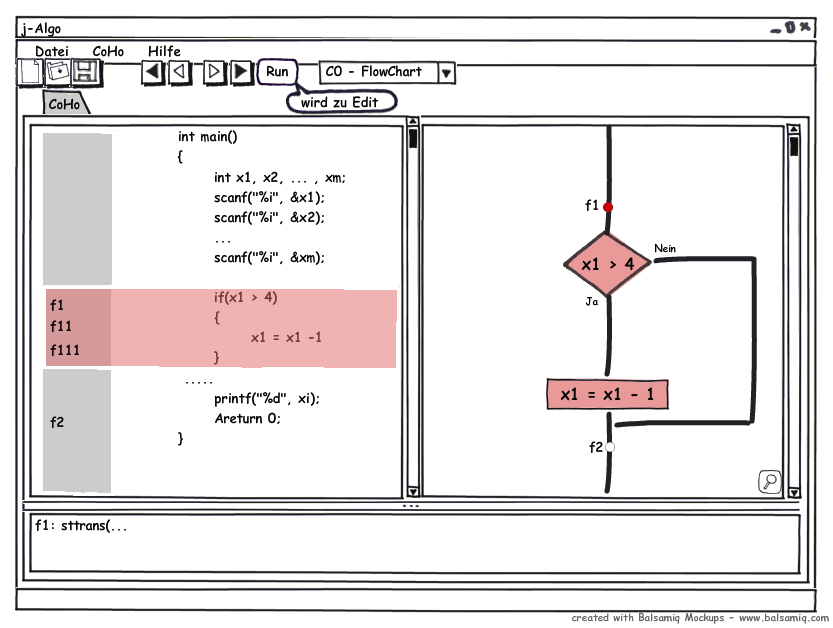
\includegraphics[scale=0.50]{images/Mockup_xml_design.png}
%	\captionof{figure}{Mockup}
\end{center}


\subsection{Workflow}
	\begin{enumerate}
		\item Willkommens-Ansicht
		\begin{description}
			Die erste Ansicht enth"alt den $C_0$-Editor im linken, sowie die Optionen im rechten Container.
			Der Benutzer w"ahlt  zuerst eine der Optionen aus dem Widget rechts aus und gelangt dann in den Editor-Modus.
		\end{description}

		\item Editor-Modus
		\begin{description}
			Hier steht einem nur das $C_0$-Code Widget zu Verf"ugung.
			Bei Bet"atigung des Run-Buttons wird der Code evaluiert und es wird gegebenenfalls in den Umwandlungs-Modus gewechselt.
		\end{description}

		\item Umwandlungs-Modus
		\begin{description}
			Im Umwandlungs-Modus ist der $C_0$-Code nicht mehr editierbar.
			Der Code kann schrittweise oder auch sofort vollst"andig durchlaufen werden, wobei er entsprechend
			in ein Flussdiagramm bzw. in $H_0$-Code umgewandelt wird.
			Ebenso ist es m"oglich, das Flussdiagramm in $H_0$-Code umzuwandeln.
		\end{description}
	\end{enumerate}
	


\subsection{Widgets}
	\subsubsection{Optionen}
		Dieser Teil orientiert sich optisch an anderen j-Algo-Modulen (z. B. KMP, AVL oder Hoare), 
		ist allerdings nur in der rechten H"alfte eingeblendet und bietet folgende Optionen:
		\begin{enumerate}
			\item "Offnen von $C_0$-Dateien
			\item "Offnen von Lehrbeispielen
			\item Eingabe der m-k-i-Parameter f"ur den $C_0$-Code
		\end{enumerate}

	\subsubsection{$C_0$-Editor}
		\begin{description}
			Dieser ist im Editor-Modus ein reiner Texteditor.
			Im Umwandlungs-Modus wird der Code formatiert und die Textbl"ocke werden semantisch hervorgehoben.
			Zus"atzlich werden baumstrukturierte Adressen angezeigt.
			Durch Anklicken werden korrespondierende Stellen in anderen Widgets hervorgehoben.
		\end{description}

	\subsubsection{Flussdiagramm}
		\begin{description}
			Dieses entspringt dem Beispiel aus dem Skript.
			Die baumstrukturierten Adressen werden an Knotenpunkten eingeblendet.
			Durch Anklicken werden korrespondierende Stellen in anderen Widgets hervorgehoben.
		\end{description}

	\subsubsection{$H_0$-Ansicht}
		\begin{description}
			Diese enth"alt den generierten $H_0$-Code.
			Durch Anklicken werden korrespondierende Stellen in anderen Widgets hervorgehoben.
		\end{description}	

	\subsubsection{Transformationsschritte}
		\begin{description}
			Hier werden die im Skript erw"ahnten "Ubersetzungsregeln bei Ausf"uhrung dargestellt.
		\end{description}

 \newpage
%  \section{Entwicklungsumgebung}

%\comment{Welche Software, Hardware und Orgware wird zur Entwicklung ben"otigt?}

\subsection{Software}
	
\begin{itemize}

	\item IDE: Eclipse
	\item Gforge Plattform
	\item dokuwiki
	\item git, svn
	\item Windows, Linux
	\item BalsamiQ

\end{itemize}

\subsection{Hardware}
\begin{itemize}
	\item Plattformunabh"angig dank JavaVM
	\item Bedienung durch Touchscreen
	\item Beamer
\end{itemize}
 \newpage
%  \section{Erg"anzungen}

%\comment{Spezielle, noch nicht abgedeckte Anforderungen.}
 \newpage
  \section{Glossar}

%\comment{Definition aller wichtigen Begriffe zur Sicherstellung einer einheitlichen Terminologie.}

\begin{description}
  \item[j-Algo]
    j-Algo ist ein an der Informatik-Fakult"at der TU-Dresden entwickeltes Programm zur Visualisierung von Algorithmen.
  \item[Modul]
    Erweiterung f"ur j-Algo
  \item[$C_0$]
    Programmiersprache, vereinfachtes C entsprechend der Vorlesung
  \item[$H_0$]
    Programmiersprache, vereinfachtes Haskell entsprechend der Vorlesung
  \item[Transformation]
    Umwandlung von $C_0$-Code in entsprechenden $H_0$-Code oder in ein Flussdiagramm nach bestimmten Regeln
  \item["Ubersetzung]
    entspricht der Transformation
  \item[Flussdiagramm]
    grafische Darstellung des eingegebenen Programms
  \item[Editor]
    Textfeld zur Eingabe von $C_0$-Code
  \item[Widget]
    Element der Benutzeroberfl"ache: $C_0$-Code, $H_0$-Code, Flussdiagramm oder Willkommens-Ansicht 
  \item[Formatierung]
    Einr"uckungen, Zeilenumbr"uche und Freir"aume werden entsprechend der Vorlesung standardisiert
\end{description}
\end{document}
